\documentclass[12pt]{article}

\usepackage{xcolor}
\usepackage{float}
\usepackage{graphicx}
\usepackage{fancyhdr}

\usepackage[utf8]{inputenc}
\usepackage{setspace}

\usepackage[dvips,letterpaper,margin=1in]{geometry}

\setlength{\parindent}{0pt}
\setlength{\headheight}{15pt} % fancyhdr wants at least 14.5pt

% Header
\pagestyle{fancy}
\lhead{MFRFS K3 Xeon-D Interface Description}
\rhead{July 28, 2020}
\renewcommand{\headrulewidth}{0.4pt}
\renewcommand{\footrulewidth}{0.4pt}

% Start document
\begin{document}

%%%%%%%%%%%%%%%%%%%% Title Page %%%%%%%%%%%%%%%%%%%%%%%%
\thispagestyle{empty}
\begin{titlepage}
\begin{center}
        \vspace*{1cm}

        \LARGE{Multi-Function Radio Frequency System (MFRFS) K3 \\
            Xeon-D Interface Description}

        \vspace{0.5cm}
        \LARGE
        % Subtitle

        \vspace{1.5cm}

        \normalsize

        John Jesus \\
        July 28, 2020

        \vfill



        \vspace{0.8cm}




\end{center}
\end{titlepage}

\tableofcontents
\newpage

%%%%%%%%%%%%%%%%% Start of Body %%%%%%%%%%%%%%%%%%%%%%%%
\section{Scope}
\subsection{Purpose}
This document is describes interfaces to the Xeon-D SoC of
the XES Xpedite7674 Single Board Computer as planned for MFRFS K3.

\subsection{References}
\begin{enumerate}
    \item XPedite7674 Users Manual Revision C (Extreme Engineering Solutions, February 1, 2018) \label{ref:board_man}
    \item XIt1088 User’s Manual Revision A (Extreme Engineering Solutions, May 29, 2019) \label{ref:rtm_man}
    \item XPEDITE7674 Schematic Diagram SCH90030490 Revision C (Extreme Engineering Solutions, February 28, 2020) \label{ref:schematic}
    \item Mercury Systems TRRUST-Stor SSD MSD256/512 and MDR256/512 (Mercury Systems, July 25, 2016) \label{ref:mercurty_ssd}
\end{enumerate}

\section{Interfaces}

Interfaces are depicted in Figure \ref{fig:inteface}.  Details of each
interface are provided in subsections below.

\begin{figure}[H]
\begin{center}
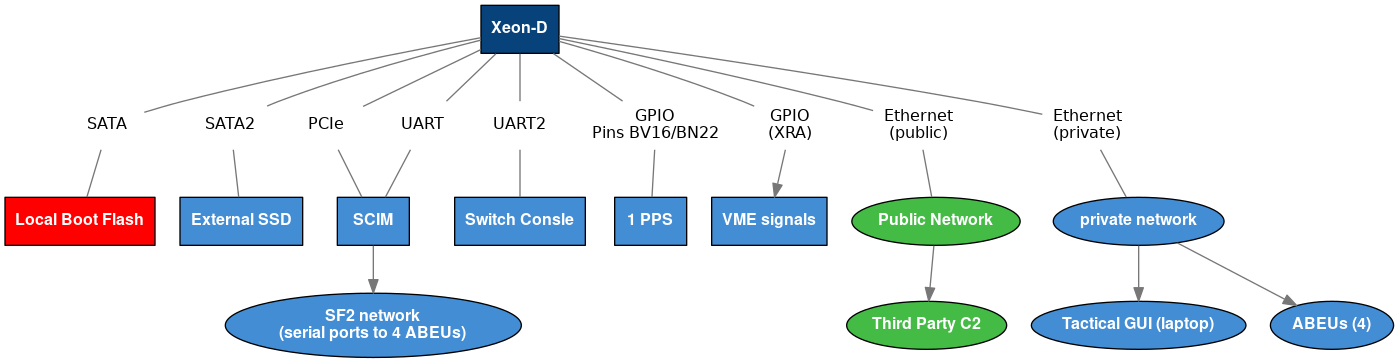
\includegraphics[width=1.0\textwidth]{img/interface}
\caption{Xeon-D Interfaces on the XPedite7674 for MFRFS K3}
\label{fig:inteface}
\end{center}
\end{figure}


% %%%%%%%%%%%%%%%%%%%%%%%%%%%%%%%%%%%%%%%%%%%%%%%
% sata (boot flash)
% %%%%%%%%%%%%%%%%%%%%%%%%%%%%%%%%%%%%%%%%%%%%%%%

\subsection{SATA (local boot flash)}
\label{section:sata}

This SATA interface is to the Linux boot image and initial ram disk.
The K3 application does not use this interface.
The only tie between the Linux boot image and the K3 application is 
an entry in the initial ram disk in \texttt{/etc/services.d} that
starts a K3 executable called \texttt{CSWMain}.
\texttt{CSWMain} is a shim program that loads configuration files
and libraries from the External SSD (Section \ref{section:sata2}) and
launches them.


% %%%%%%%%%%%%%%%%%%%%%%%%%%%%%%%%%%%%%%%%%%%%%%%
% sata2 (external ssd)
% %%%%%%%%%%%%%%%%%%%%%%%%%%%%%%%%%%%%%%%%%%%%%%%

\subsection{SATA (External SSD)}
\label{section:sata2}

An External Solid-State Drive (SSD) is the Mercury Systems TRRUST-Stor SSD MSD512 Self-Encrypted Drive mounted in a 3-U carrier in Slot 8 of the VPX chassis.  The Xeon-D has a SATA connection to this SSD through the VPX backplane and uses the serial port interface through the SCIM (Figure \ref{fig:ssd}) to send key information to unlock the SSD. 
%%%
\vspace{0.8cm}

\begin{figure}[H]
\begin{center}
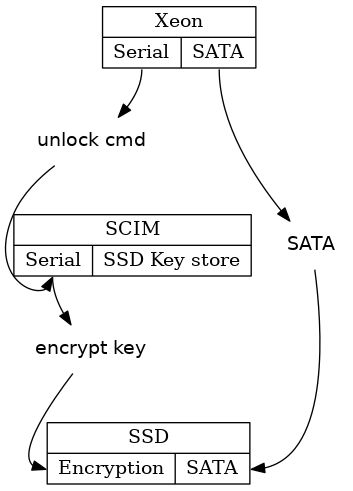
\includegraphics[width=0.3\textwidth]{img/ssd}
\caption{External SSD, Self-Encrypted}
\label{fig:ssd}
\end{center}
\end{figure}

\textcolor{red}{\textbf{Question for Nick:} Do you think we need to
continue using a Self-Encrypted Drive like the Mercury TRRUST-Stor?}

%%%

% %%%%%%%%%%%%%%%%%%%%%%%%%%%%%%%%%%%%%%%%%%%%%%%
% switch console
% %%%%%%%%%%%%%%%%%%%%%%%%%%%%%%%%%%%%%%%%%%%%%%%

\subsection{Serial Port to Ethernet Switch Console}
\label{section:switch_console}

The Xeon has a serial port connection to the console of the Ethernet switch that has ports for both internal Ethernet and the public classified Ethernet.
The purpose of this connection is for application software to act as a "terminal scraper" and enter switch maintenance commands to configure/reconfigure the network, for example, creating separate VLANs for each of the internal and public networks.

\textcolor{red}{\textbf{Question for Nick:} How \textit{robust} (not the word I really mean to use) is this connection and use-case?}


% %%%%%%%%%%%%%%%%%%%%%%%%%%%%%%%%%%%%%%%%%%%%%%%
% 1 PPS
% %%%%%%%%%%%%%%%%%%%%%%%%%%%%%%%%%%%%%%%%%%%%%%%

\subsection{PPS signal}
\label{section:pps}

The pulse-per-second signal is transferred from the ETalin/GPS through discrete lines on the SCIM and appears on a GPIO pin on the Xeon that is serviced by an IRQ.
This interrupt seems to be used by the \textit{Chrony} facility (\textit{Chrony} is an alternative to \textit{NTP}).


\textcolor{red}{\textbf{Question for Nick:} Is it OK that this line does not go through the Kintex?}


% %%%%%%%%%%%%%%%%%%%%%%%%%%%%%%%%%%%%%%%%%%%%%%%
% Slot number and system id
% %%%%%%%%%%%%%%%%%%%%%%%%%%%%%%%%%%%%%%%%%%%%%%%

\subsection{Slot number and System ID}
\label{section:slot_system_id}

These signals are literally hard-wired static signals from the VME backplane that can be read on the Xeon through I\textsuperscript{2}C interface to an XRA GPIO Expander.
The slot id is inferred from the VME geographic address pins (which are grounded in the backplane connector) and the System ID (\textit{K2} / \textit{K3} / \textit{XBEAU}) is inferred from strapping elsewhere on the backplane.

% %%%%%%%%%%%%%%%%%%%%%%%%%%%%%%%%%%%%%%%%%%%%%%%
% Internal Ethernet
% %%%%%%%%%%%%%%%%%%%%%%%%%%%%%%%%%%%%%%%%%%%%%%%

\subsection{Internal Ethernet}
\label{section:internal_ethernet}

The Xeon is on the main board in the System Controller Unit (SCU).  Ethernet hosts on the network are:

Single-Board Computer cards in the Array Back-End Units (ABEU)



% %%%%%%%%%%%%%%%%%%%%%%%%%%%%%%%%%%%%%%%%%%%%%%%
% External Ethernet
% %%%%%%%%%%%%%%%%%%%%%%%%%%%%%%%%%%%%%%%%%%%%%%%

\subsection{External Ethernet}
\label{section:external_ethernet}


\end{document}

